\chapter[Langages algébriques]{Grammaires hors contexte et langages algébriques}
\label{chp.alg}

\minitoc

\lettrine{D}{ans} le chapitre précédent, nous avons étudié les expressions
rationnelles. Celles-ci sont particulièrement simples~: leur forme est limitée
à l'étoile, l'union et la concaténation. On a vu par exemple que le langage
$\{a^nb^n\}_{n\in\bN}$ n'est pas rationnel. Un tel langage paraît pourtant
intéressant, d'où la volonté de construire un formalisme plus riche que celui
des expressions rationnelles.

Les langages algébriques, encore appelés langages hors contextes, sont des
langages nés d'un tel formalisme. Ce chapitre est dédié à l'étude de ce
formalisme, qui est celui des grammaires hors contexte. Nous verrons ces
grammaires ainsi que les automates associés aux langages algébrique~: les
automates à pile. Contrairement aux automates finis, les automates à pile ont
une forme de mémoire, grâce à une pile de symboles.

\section{Grammaire hors contexte}\label{sec.alg1}

Le formalisme des grammaires hors contexte est particulièrement proche des
fondements de l'informatique~: c'est par exemple ce formalisme qui est utilisé
pour décrire des langages de programmation.

L'idée d'une grammaire est de permettre de construire des mots en utilisant des
règles de formation. Pour donner un exemple, essayons de générer une expression
arithmétique~: une telle expression est une somme, un produit ou un entier. Une
première tentative est donc d'utiliser des BNF, comme au \cref{chp.induction},
ce qui donne alors~:
\[e,e' \inddefeq n \mid e + e' \mid e \times e'\]
Un souci apparaît alors~: comment lire $2 + 3 \times 4$ ? Dans les premiers
chapitres, nous avons décidé de considérer que dans un tel cas, il y a deux
expressions possibles $(2 + 3) \times 4$ et $2 + (3 \times 4)$ et l'une des deux
est privilégiée par des règles de priorité. Une autre façon de faire, qui est
celle que l'on formalise à l'aide des grammaires hors contexte, est d'inclure
explicitement le parenthésage dans la construction d'une expression. En faisant
cela, on souhaite obtenir une description de nos expressions uniquement comme
un sous-ensemble de $(\bN \cup \{(,),+,\times\})^\star$.

\begin{remark}
  En réalité, on parle aussi de BNF dans le cas de la présentation qui sera
  donnée dans la suite de ce chapitre des grammaires hors contextes. Dans ce
  livre, on considérera toutefois qu'une BNF sera une spécification moins
  formelle d'un ensemble inductif. On gardera l'expression \og grammaire hors
  contexte\fg{} dans le cas où l'on veut parler d'un ensemble de mots décrit par
  des règles syntaxiques.
\end{remark}

\subsection{Premières définitions}

Donnons directement la définition d'une grammaire hors contexte, qui est l'objet
que nous manipulerons pour le reste de la \cref{sec.alg1}. Comme nous
n'utiliserons par d'autres grammaires ici, on parlera directement de grammaire
pour signifier \og grammaire hors contexte\fg{}.

\begin{definition}[Grammaire hors contexte]
  Soit $\ABA$ un alphabet. On appelle grammaire hors contexte sur $\ABA$ un
  triplet $(\ABB,\to,\StGr)$ où $\ABB$ est un alphabet disjoint de $\ABA$,
  $\mathord{\to}\subseteq \ABB\times \toSt{(\ABA \cup \ABB)}$ et
  $\StGr \in \ABB$. Dans ce cadre, on appelle les éléments de $\ABB$ des
  symboles non terminaux (ou simplement des non terminaux) et les éléments de
  $\ABA$ des symboles terminaux (ou simplement des terminaux). On appelle $\to$
  les règles de la grammaire. Chaque élément $(\varwd,\varwv)\in\mathord{\to}$
  est appelé une règle de la grammaire. On note $\Gram(\ABA)$ l'ensemble des
  grammaires hors contexte sur $\ABA$.
\end{definition}

\begin{notation}
  Dans le contexte des grammaires formelles, on va noter les non terminaux par
  des majuscules $\nTA,\nTB\ldots$ et conserver les symboles
  $\varla,\varlb\ldots$ pour désigner les terminaux.
\end{notation}

Une grammaire hors contexte consiste donc en la donnée des symboles qui seront
d'intérêt, d'un symboles de départ donné et de règles permettant de construire
des mots en remplaçant des symboles non terminaux. On souhaite pouvoir, par
exemple, faire la réécriture
\[\nTE + 3 \to 2 + 3\]
pour remplacer le non terminal $\nTE$ (représentant une expression) en le
terminal $2$. Cela nous mène donc à la notion de dérivation.

\begin{definition}[Dérivation]
  Soit une grammaire $\varGG$. On appelle dérivation en un pas de
  $\varwd \in \toSt{(\ABA\cup \ABB)}$ vers
  $\varwd' \in \toSt{(\ABA\cup\ABB)}$ la
  relation, qu'on notera aussi $\varwd \to \varwd'$, définie par le fait qu'il
  existe une décomposition de $\varwd$ et $\varwd'$ de la forme
  \[\begin{cases}
  \varwd = \varwv \nTA\varww\\
  \varwd' =\varwv \varwx\varww
  \end{cases}\]
  où $\nTA \to \varwx$, c'est-à-dire $(\nTA,\varwx) \in \mathord{\to}$. On
  appelle dérivation de $\varwd$ vers $\varwd'$ la clôture réflexive et
  transitive $\rtClot{\to}$ de la dérivation en un pas.
\end{definition}

\begin{remark}
  On parlera indifféremment de dérivation de $\varwd$ vers $\varwv$ pour la
  relation $\varwd \rtClot{\to} \varwv$ et pour une suite
  $\varwd_0,\ldots,\varwd_n$ telle que $\varwd_0 = \varwd$,
  $\varwd_n = \varwv$ et $\forall i \in \intervInt{n},\varwd_i \to \varwd_{i+1}$.
  L'existence d'une telle suite étant équivalente à $\varwd \rtClot{\to}\varwv$,
  cet abus de langage ne pose aucun problème au niveau logique.
\end{remark}

\begin{exercise}[Définition alternative d'une dérivation]
  Soit $\ABA$ un alphabet et $\varRR$ une relation sur $\toStA$. On dit que
  $\varRR$ est compatible si cette relation vérifie
  \[\forall \varwd_0,\varwv,\varwv',\varwd_1\in\toStA,
  \varwv\varRR\varwv' \implies
  \varwd_0\varwv\varwd_1\varRR\varwd_0\varwv'\varwd_1\]
  Montrer que la relation de dérivation est la plus petite relation sur
  $\toSt{(\ABA\cup\ABB)}$ compatible et contenant les règles de la grammaire.
\end{exercise}

Nous introduisons quelques règles de notations pour rendre les définitions de
grammaires plus lisibles.

\begin{notation}
  Pour décrire une grammaire, on précisera son alphabet $\ABA$, mais $\ABB$
  restera implicite~: on déduit $\ABB$ de l'ensemble des non terminaux utilisés
  lors de l'écriture des règles. Pour écrire les règles, on donnera la syntaxe
  suivante~:
  \begin{align*}
    \StGr &\to \varwd_1\mid \cdots\mid \varwd_n\\
    \nTA &\to \varwv_1\mid\cdots\mid \varwv_p\\
    &\vdots
  \end{align*}
  On notera toujours $\StGr$ pour l'élément $\StGr \in \ABB$. De plus, en
  pratique, on pourra utiliser des mots-clés plutôt que des lettres comme
  éléments de $\ABB$~: cela permet de clarifier les constructions, mais du côté
  théorique on suppose que ces mots-clés sont simplement des symboles.
\end{notation}

Donnons maintenant deux exemples fondamentaux~: les expressions arithmétiques et
les mots de Dyck.

\begin{example}
  On définit la grammaire $\varGG_{\Arith}$ comme suit~:
  \begin{itemize}
  \item $\ABA = \{0,\Ss,(,),+,\times\}$
  \item Les règles sont~:
    \[\begin{array}{lcl}
    \StGr & \to & \MultExp + \StGr \mid \MultExp\\
    \MultExp & \to & \Atom \times \MultExp \mid \Atom\\
    \Atom & \to & 0 \mid \Ss\Atom \mid (\StGr)
    \end{array}\]
  \end{itemize}
  
  On définit la grammaire $\varGG_D$ comme suit~:
  \begin{itemize}
  \item $\ABA = \btwo$
  \item Les règles sont~:
    \begin{align*}
      \StGr &\to \StGr 0\StGr 1\mid\Ewd
    \end{align*}
  \end{itemize}
\end{example}

Donnons aussi des exemples de dérivations, en utilisant nos deux premières
grammaires. Une première dérivation, dans $\varGG_{\mathrm{arith}}$~:
\begin{align*}
  \StGr &\to \MultExp + \StGr \to \MultExp + \MultExp \\
  &\to \Atom + \MultExp \to \Atom + \Atom \times \MultExp \\
  &\to \Ss\Atom + \Atom\times \MultExp \\
  &\to \Ss\Ss\Atom + \Atom\times \MultExp \\
  &\to \Ss\Ss 0 + \Atom\times\MultExp \\
  &\to 2 + (\StGr)\times \MultExp \to
  2 + (\StGr) \times \Atom \to^4 2 + (\StGr) \times 3\\
  &\to 2 + (\MultExp) \times 3 \to 2 + (\Atom \times \MultExp) \times 3\\
  &\to^5 2 + (4 \times \MultExp) \times 3\\
  &\to^6 2 + (4 \times 5) \times 3
\end{align*}
où on remplace $\Ss^n 0$ par $n$, pour garder une forme de lisibilité.

Une autre dérivation, dans $\varGG_D$~:
\begin{align*}
  \StGr &\to \StGr 0\StGr 1 \to \StGr 0\StGr 10\StGr 1 \to 0\StGr 10\StGr 1
  \to 0\StGr 0\StGr 110\StGr 1 \to 00\StGr 110\StGr 1 \\
  &\to 00\StGr 110\StGr 0\StGr 11 \to 00\StGr 1100\StGr 11
  \to 00\StGr 1100\StGr 0\StGr 111\to 00\StGr 11000\StGr 111\\
  &\to^2 0011000111
\end{align*}

Dans ces deux dérivations, nous voyons une différence importante entre le mot
final et les mots précédents~: le mot final ne contient plus de symbole non
terminal (d'où l'utilisation du mot \og terminal\fg). On a ainsi deux notions de
langages qui sont naturellement associées à une grammaire.

\begin{definition}[Langage engendré par une grammaire]
  Soit $\varGG$ une grammaire. On définit les deux langages engendrés par
  $\varGG$~:
  \[\widehat{\varLL_{\varGG}}\defeq
  \compr{\varwd \in \toStAB}{\StGr\rtClot{\to} \varwd} \qquad
  \varLL_{\varGG} \defeq \widehat{\varLL_{\varGG}}\cap \toStA\]
  Lorsque l'on parle du langage engendré par $\varGG$, on désigne l'ensemble
  $\varLL_{\varGG}$.
\end{definition}

\begin{definition}[Langage hors contexte]
  Soit $\ABA$ un alphabet. On appelle classe des langages algébrique (ou hors
  contexte) la classe de langages sur $\ABA$ définie par
  \[\varCC_{\alg}\defeq \compr{\varLL_{\varGG}}{\varGG\in\Gram(\ABA)}\]
\end{definition}

\begin{remark}
  L'expression \og hors contexte\fg vient du fait que les grammaires que nous
  utilisons n'utilisent que des règles sans contexte d'application~: on se
  contente de remplacer des non terminaux dès qu'ils apparaissent, mais on n'a
  pas de règles telles que, par exemple~:
  \[\varwd\nTA\nTA \to \nTC\nTB\nTA\]
  où plusieurs symboles apparaissent à gauche de $\to$ et forcent donc à avoir
  un contexte de dérivation.
\end{remark}

\begin{exercise}
  Soit un alphabet $\ABA$. Montrer que le langage des palindromes sur $\ABA$,
  c'est-à-dire l'ensemble
  \[\varLL_{\palindrome} \defeq
  \compr{\varwd \in \toStA}
        {\forall i \in \intervInt{\wul},\varwd_i = \varwd_{\wul - i}}\]
  est un langage algébrique. Est-il rationnel ?
\end{exercise}

Un point essentiel avec les grammaires hors contextes est que, comme la seule
donnée importante lors d'une dérivation est le symbole que l'on décide de
dériver, il est possible de séparer des dérivations en coupant arbitrairement un
mot. Cela nous mène au lemme suivant, qualifié de fondamental dans
\cite{carton2008langages}.

\begin{lemma}
  Soit un alphabet $\ABA$, une grammaire $\varGG$ sur $\ABA$ et
  $\varwd \in \toStAB$. Il existe alors une dérivation $\varwd \to^k \varwv$
  de longueur $k$ vers un mot $\varwv \in \toStAB$ si et seulement s'il existe
  deux décompositions
  \[\begin{cases}
  \varwd = \varwd_1\wdPt \varwd_2 \\
  \varwv = \varwv_1\wdPt \varwv_2
  \end{cases}\]
  et deux dérivations
  \[ \varwd_1 \to^{k_1} \varwv_1 \qquad \varwd_2 \to^{k_2} \varwv_2\]
  telles que $k_1 + k_2 = k$.
\end{lemma}

\begin{proof}
  Dans un sens, prenons deux dérivations $\varwd_1 \rtClot{\to} \varwv_1$ et
  $\varwd_2\rtClot{\to} \varwv_2$. Comme on peut former la dérivation
  $\varwd_1 \wdPt \varwd_2 \rtClot{\to} \varwv_1 \wdPt \varwd_2\rtClot{\to}
  \varwv_1 \wdPt \varwv_2$,
  une récurrence sur $k_1$ et $k_2$ nous permet de déduire qu'on peut composer
  deux dérivations parallèles.

  Dans l'autre sens, on procède par récurrence sur $k$ pour montrer que si
  $\varwd \to^k \varwv$ alors il existe une décomposition
  $\varwv = \varwv_1\wdPt \varwv_2$ et $k_1,k_2$
  tels que $k_1+k_2 = k$, $\varwd_1\to^{k_1} \varwv_1$ et
  $\varwd_2\to^{k_2}\varwv_2$~:
  \begin{itemize}
  \item dans le cas où $\varwd \to^0 \varwd$, on pose
    \[\varwv_1\defeq \varwd_1 \qquad \varwv_2 \defeq \varwd_2\]
    et on a le résultat.
  \item supposons que l'implication est vraie pour $k$. Si on a une dérivation
    $\varwd \to^{k+1} \varwv$, alors on peut trouver $\varww$ tel que
    $\varwd \to^k \varww \to \varwv$, et décomposer $\varww$ en
    $\varww_1\wdPt \varww_2$, de telle sorte que
    \[\varwd_1 \to^{k_1} \varww_1 \qquad \varwd_2 \to^{k_2} \varww_2\]
    et $k_1 + k_2 = k$. De plus, on sait par définition de $\varww \to \varwv$
    qu'il existe une lettre de $\varww$ qui sera remplacée en appliquant une
    règle de notre grammaire. Cette lettre est soit dans $\varww_1$, auquel cas
    on pose $\varwv_1$ le résultat de cette dérivation en $\varww_1$ et
    $\varwv_2 \defeq \varww_2$ pour obtenir le résultat, soit dans $\varww_2$ et
    un raisonnement analogue s'applique.\qedhere
  \end{itemize}
\end{proof}

\subsection{Grammaires sous formes particulières}

Pour manipuler des grammaires, il est souvent utile de les transformer pour leur
donner une forme plus pratique. Nous allons ici traiter de quatre formes
importantes que peuvent avoir des grammaires~: la forme réduite, la forme
propre, la forme normale de Chomsky et la forme normale de Greibach.

Nous reprenons assez directement les preuves données dans
\cite{carton2008langages}, et décidons donc de conserver la mise en avant de la
possibilité d'implémenter de vrais algorithmes à partir des preuves données.

Dans le cas des automates, nous avons vu qu'il était possible de considérer des
automates émondés, c'est-à-dire tels que tout état est à la fois accessible et
co-accessible. Dans le cas d'une grammaire, la notion analogue est celle de
forme réduite~: toute variable dans $\ABB$ peut apparaître dans une dérivation
produisant un mot.

\begin{definition}[Forme réduite]
  Soit $\ABA$ un alphabet. On dit qu'une grammaire $(\ABB,\to,\StGr)$ sur $\ABA$
  est sous forme réduite si les deux conditions suivantes sont vérifiées~:
  \begin{itemize}
  \item pour tout $\nTA \in \ABB$, il existe $\varwd\in\toStA$ tel que
    $\nTA \toSt{\to} \varwd$.
  \item pour tout $\nTA \in \ABB$, il existe $\varwd,\varwv\in\toStAB$ tels que
    $\StGr \toSt{\to} \varwd\nTA\varwv$.
  \end{itemize}
\end{definition}

Comme avec les automates, il est possible de se ramener à une grammaire sous
forme réduite sans changer le langage engendré.Cela justifie aussi notre
présentation des grammaire dans laquelle l'alphabet $\ABB$ se déduit des
symboles utilisés dans les règles.

\begin{proposition}\label{prop.alg.reduc}
  Soit un alphabet $\ABA$ et une grammaire $\varGG=(\ABB,\to,\StGr)$. Il existe
  $\ABB'\subseteq\ABB$ tel que, en notant $\varGG'=(\ABB',\to,\StGr)$, $\varGG'$
  est sous forme réduite et $\varLL_{\varGG} = \varLL_{\varGG'}$.
\end{proposition}

\begin{proof}
  Pour construire notre nouvelle grammaire, on procède en éliminant des symboles
  ne respectant pas la condition de réduction. On construit donc un nouvel
  ensemble de symboles $\ABD \subseteq \ABA\cup\ABB$ par la suite suivante~:
  \[\begin{cases}
  \ABD_0 \defeq \ABA \\
  \ABD_{n+1} \defeq \ABD_n \cup
  \compr{\nTA \in \ABB}{\nTA \to \varwd \land \varwd \in \toSt{(\ABD_n)}}
  \end{cases}\]
  Il est clair que $(\ABD_n)$ est une suite d'ensembles finis croissante et
  majorée par $\ABA\cup \ABB$, donc elle est stationnaire. On définit donc
  $\ABD$ comme l'union des $\ABD_n$.

  On peut prouver par récurrence sur $n$ que pour tout $\nTA \in \ABB$,
  $\nTA \in \ABD_n$ si et seulement s'il existe $\varwd \in \toStA$ tel que
  $nTA \rtClot{\to} \varwd$ avec une réduction de taille inférieure à $n$, en
  utilisant la définition de $\ABD_{n+1}$~: ainsi, tout symbole dans $\ABD$ peut
  produire un mot de $\toStA$.

  On construit maintenant une deuxième suite, à partir de $\ABD$, pour
  ne considérer que les variables qui peuvent être atteintes par des dérivations
  depuis $\StGr$. On définit la suite d'ensembles finis $(\ABT_n)$ suivantes~:
  \[\begin{cases}
  \ABT_0 \defeq \{\StGr\}\\
  \ABT_{n+1} \defeq \ABT_n \cup
  \compr{\nTA \in \ABD}{\exists \nTB \in \ABT_n,
  \exists \varwd,\varwv \in \toSt{\ABD}, \nTB \to \varwd\nTA\varwv}
  \end{cases}\]
  Comme précédemment, on considère $\ABT$ l'union finie des $\ABT_n$ car on a
  une suite croissante majorée d'ensembles finis.

  On peut prouver que pour tout $\nTA \in \ABA\setminus\ABD$, $\nTA \in \ABT_n$
  si et seulement s'il existe deux mots $\varwd,\varwv \in \toSt{\ABD}$ et une
  dérivation $\StGr \rtClot{\to} \varwd\nTA\varwv$ de taille inférieure à $n$,
  dont tous les mots de la dérivation appartiennent à $\toSt{\ABD}$, là encore
  par récurrence sur $n$.

  On définit donc
  \[\ABB' \defeq \ABT\setminus \ABA\]
  et par les deux arguments précédents on sait que la grammaire induite sur
  $\ABB'$ est sous forme réduite.

  Pour montrer que les deux grammaires engendrent les mêmes mots, il nous suffit
  de montrer que toute dérivation $\StGr \rtClot{\to} \varwd$ faite dans
  $(\ABB,\to,\StGr)$ fonctionne aussi dans $(\ABB',\to,\StGr)$ (l'autre étant
  vraie par inclusion). On remarque que puisque la dérivation ne contient que
  des non terminaux qui peuvent produire un mot, tous les non terminaux
  apparaissant dans la dérivation $\StGr \rtClot{\to} \varwd$ sont des éléments
  de $\ABD$. De plus, ils sont clairement dans $\ABT$, donc ils sont dans
  $\ABB'$. On en déduit l'égalité des deux langages.
\end{proof}

\begin{remark}
  Les définitions de $(\ABD_n)$ et $(\ABT_n)$ donnent un algorithme pour trouver
  les états à conserver pour avoir une grammaire sous forme réduite. Si l'on
  souhaite implémenter ces suites d'ensembles, il faut aussi se demander comment
  tester à quel moment ces deux suites se stabilisent~: on voit en fait que dès
  que $\ABD_{n+1} = \ABD_n$ (respectivement $\ABT_{n+1}=\ABT_n$) alors la suite
  devient stationnaire. Il suffit donc de vérifier lors de la construction de
  $\ABD_{n+1}$ (respectivement de $\ABT_{n+1}$) si des éléments ont été ajoutés ou
  non.
\end{remark}

La deuxième forme à introduire est la forme propre. Celle-ci permet d'éliminer
des règles qui rallongent artificiellement les dérivations. On peut y voir un
analogue d'un automate sans $\Ewd$-transition~: chaque règle dans une grammaire
sous forme propre produit effectivement un terminal ou deux non terminaux.

\begin{definition}[Forme propre]
  Soit $\ABA$ un alphabet. Une grammaire $(\ABB,\to,\StGr)$ sur $\ABA$ est dite
  sous forme propre s'il n'existe aucune règle de la forme $\nTA \to \Ewd$ ni
  $\nTA \to \nTB$ où $\nTA,\nTB\in\ABB$.
\end{definition}

Si l'on souhaite mettre une grammaire sous forme propre, il semble que dériver
le mot $\Ewd$ devient impossible~: c'est effectivement le cas, mais il est
possible de passer une grammaire sous forme propre en ne perdant que ce
potentiel mot. Nous utilisons la notion de substitution pour rendre plus lisible
la construction d'une grammaire sous forme propre.

\begin{definition}[Substitution]\label{def.ghc.subst}
  Soient $\ABA, \ABB$ deux alphabets. On appelle substitution de $\ABA$ vers
  $\ABB$ un morphisme de monoïde
  $\makeFunName{\subSimul}{\toStA}{\powerset (\toStB)}$ où $\powerset(\toStB)$
  est muni de la loi de produit des langages (et du langage $\{\Ewd\}$ comme
  élément neutre).
\end{definition}

\begin{proposition}
  Soit $\ABA$ un alphabet et $\varGG=(\ABB,\to,\StGr)$ une grammaire sur $\ABA$.
  Alors il existe une grammaire $\varGG'$ sur $\ABA$ sous forme propre telle que
  $\varLL_{\varGG'} = \varLL_{\varGG} \setminus \{\Ewd\}$.
\end{proposition}

\begin{proof}
  Tout d'abord, on suppose (quitte à utiliser la \cref{prop.alg.reduc}) que
  notre grammaire est sous forme réduite.

  On commence par chercher à supprimer les règles de la forme $\nTA \to \Ewd$.
  Pour cela, on introduit d'abord l'ensemble $\ABD$ des symboles qui peuvent
  produire $\Ewd$, en donnant la suite $(\Delta_n)$ suivante~:
  \[\begin{cases}
  \ABD_0 \defeq \compr{\nTA \in \ABB}{\nTA \to \Ewd}\\
  \ABD_{n+1} \defeq \ABD_n \cup
  \compr{\nTA\in\ABB}{\exists \varwd \in\toSt{(\ABD_n)}, \nTA \to \varwd}
  \end{cases}\]
  Comme cette suite est stationnaire (toujours par les mêmes arguments), on
  définit $\ABD$ l'union croissante finie de ces ensembles. On peut montrer par
  récurrence que $\Delta_n$ est exactement l'ensemble des symboles $\nTA\in\ABB$
  tels que $\nTA \rtClot{\to} \Ewd$. On définit maintenant la substitution de
  $\ABA\cup\ABB$ dans lui-même en donnant l'image de chaque élément de
  $\ABA\cup\ABB$ (et en étendant cette fonction à $\toSt{(\ABA\cup\ABB)}$ par le
  \cref{thm.PU.monoid})~:
  \[\begin{cases}
  \subSimul(\varla) \defeq \{\varla\} \text{ si } \varla \in \ABA\\
  \subSimul(\nTA) \defeq \{\nTA , \Ewd\} \text{ si } \nTA \in \ABD\\
  \subSimul(\nTA) \defeq \{\nTA\} \text{ si } \nTA \in\ABB\setminus\ABD
  \end{cases}\]

  Cette substitution nous permet de retenir quels mots doivent être ajoutés
  lorsque l'on supprime les règles $\Ewd$. En effet, si l'on supprime
  directement chaque règle de la forme $\nTA \to \Ewd$, on risque de perdre des
  dérivations qui feraient intervenir une dérivation de cette forme, entourée
  d'autres dérivations. On décide donc d'ajouter à nos règles toutes les règles
  de la forme $\nTA\to\varwd$ où $\varwd$ a été obtenu par une dérivation depuis
  $\nTA$ qui fait potentiellement apparaître un $\Ewd$.

  On définit donc la relation $\to'$ comme la plus petite relation qui contient
  $\to$ privé de l'ensemble $\compr{(\nTA,\Ewd)}{\nTA\in\ABB}$, et qui contient
  chaque règle $\nTA \to' \varwd$ où $\nTA \to \varww$ et
  $\varwd \in \subSimul(\varww)\setminus\{\Ewd\}$ (comme l'ensemble des règles
  $\nTA \to \varww$ est fini, l'ensemble des règles ajoutées dans $\to'$ est lui
  aussi fini).

  On veut prouver qu'un mot non vide est dérivable pour une relation si et
  seulement s'il l'est pour l'autre.

  Commençons par prouver que si $\nTA \to' \varwd$, alors
  $\nTA \rtClot{\to} \varwd$ dans le cas où $\varwd \neq \Ewd$. Pour cela, il
  nous suffit de montrer que pour toute règle $\nTA \to \varww$ et
  $\varwd\in\subSimul(\varww)\setminus\{\Ewd\}$, on a $\nTA\rtClot{\to}\varwd$.
  Pour cela, on procède par récurrence sur la taille de $\varww$~:
  \begin{itemize}
  \item si $\nTA \to \varww$ et $\varww = \Ewd$, alors
    $\varwd \in \subSimul(\varww)\setminus\{\Ewd\}$ est absurde, donc le cas est
    traité.
  \item supposons que $\nTA \rtClot{\to}\varwd$ pour tout $\nTA$ et tout
    $\varwd \in \subSimul(\varww)\setminus\{\Ewd\}$ avec $\varww$ de taille $n$
    et $\nTA\to \varww$. Soit $\varww' = \varww\wdPt \varla$, où $\varla$ est
    une lettre, $\nTA$ un non terminal et
    $\varwd \in \subSimul(\varww')\setminus\{\Ewd\}$ tels que $\nTA \to\varww'$.
    On distingue deux cas~:
    \begin{itemize}
    \item si $\varla \in \ABD$, alors
      $\subSimul(\varww') = \subSimul(\varww) \cup\subSimul(\varww)\{\varla\}$,
      et on en déduit donc que soit
      $\varwd \in \subSimul(\varww)\setminus\{\Ewd\}$
      (auquel cas la propriété est vérifiée par hypothèse de récurrence), soit
      $\varwd=\varwd'\varla$ et $\varwd'\in\subSimul(\varww)\setminus\{\Ewd\}$,
      et la propriété est alors encore vérifiée.
    \item si $\varla \notin \ABD$, alors $\subSimul(\varww')=\subSimul(\varww)$,
      donc l'hypothèse de récurrence s'applique directement.
    \end{itemize}
  \end{itemize}
  Ainsi $\to'$ ne rajoute pas de mots dérivés.

  Pour le sens réciproque, il nous faut procéder par induction sur la longueur
  d'une dérivation pour prouver que si $\nTA \rtClot{\to} \varwd$ alors
  $\nTA \rtClot{\to'} \varwd$, où $\varwd$ est non vide~:
  \begin{itemize}
  \item le seul mot dérivable en $0$ étape est $\StGr$ dans les deux cas
  \item supposons l'implication prouvée pour le cas d'une dérivation en $n$
    étapes, et soient $\nTA,\varwd$ tels que $\nTA \to^{n+1} \varwd$, montrons
    que $\nTA \toSt{\to'} \varwd$. Par construction on peut considérer que
    $\nTA \to^n \varwv\nTB\varww \to \varwv\varwx\varww$ avec $\nTB \to \varwx$
    et $\varwd = \varwv\varwx\varww$. Par hypothèse d'induction, on sait
    donc que $\nTA \rtClot{\to'} \varwv\nTB\varww$~; deux cas se présentent
    alors~:
    \begin{itemize}
    \item si $\varwx = \Ewd$, alors considérons le mot $\varwd_0$ tel que
      $\varwd_0 \to \varwv\nTB\varww$. On peut le décomposer en
      $\varwd_0 = \varwv_0 \nTC\varww_0$ et décomposer nos deux mots
      $\varwv,\varww$ en $\varwv = \varwv_0 \varwv_1$ et
      $\varww = \varww_1\varww_0$.
      On voit alors que $\varwv_1\varww_1 \in \sigma(\varwv_1\nTB\varww_1)$,
      donc $\nTC\to' \varwv_1\nTB\varww_1$. Il vient finalement que
      $\varwd_0 \to' \varwx$.
    \item si $\varwx$ est non vide, alors comme $\varwx \in \subSimul(\varwd)$
      (le résultat se prouve par une induction directe sur $\varwd$, puisque
      $\subSimul(\varla)$ contient $\varla$ pour toute lettre $\varla$), on en
      déduit que $\varwv\nTB\varwv \to \varwd$.
    \end{itemize}
  \end{itemize}

  Les deux langages engendrés sont donc les mêmes, à l'exception potentielle de
  $\Ewd$.

  Il nous reste maintenant à supprimer les règles de la forme $\nTA \to \nTB$.
  Pour cela, on supprime simplement les telles règles, et on ajoute toutes les
  règles de la forme $\nTA \to \varww$ où $\nTA \rtClot{\to} \nTB$ et
  $\nTB \to \varww$. Le langage reconnu ne change donc pas.
\end{proof}

\begin{remark}
  Il est commun, dans la pratique, de ne pas avoir besoin du mot vide lorsque
  l'on utilise une grammaire hors contexte. Dans le cas par exemple des
  expressions arithmétiques, des termes sur une signature ou des formules sur
  une signature, il n'y a aucun besoin d'inclure le mot vide. On peut néanmoins
  relever des langages comme celui de Dyck contenant le mot vide.
\end{remark}

Une autre forme normale importante est celle de Chomsky. Dans la forme
précédente, on exige qu'une règle ne puisse pas avoir à droite un seul non
terminal ou $\Ewd$. Dans le forme normale de Chomsky, on impose une structure
encore plus rigide en demandant à ce les membres de droite soient toujours
un seul terminal, ou exactement deux non terminaux. On appelle aussi cette forme
la forme normale quadratique, à cause de la restriction d'avoir deux non
terminaux à droite.

\begin{definition}[Forme normale de Chomsky \cite{CHOMSKY1959137}]
  Soientt un alphabet $\ABA$ et une grammaire $\varGG=(\ABB,\to,\StGr)$ sur
  $\ABA$.
  On dit que $\varGG$ est sous forme normale de Chomsky (ou forme normale
  quadratique) lorsque toutes ses règles sont de l'une des deux formes~:
  \begin{itemize}
  \item $\nTA \to \nTB\nTC$ avec $\nTB,\nTC\in \ABB$
  \item $\nTA \to \varla$ où $\varla \in \ABA$
  \end{itemize}
\end{definition}

\begin{proposition}\label{prop.chom}
  Soient $\ABA$ un alphabet et $\varGG = (\ABA,\to,\StGr)$ une grammaire sur
  $\ABA$.
  Il existe une grammaire $\varGG'$ sous forme normale de Chomsky telle que
  $\varLL_{\varGG'} = \varLL_{\varGG}\setminus \{\Ewd\}$.
\end{proposition}

\begin{proof}
  On commence par supposer que $\varGG$ est sous forme propre (d'où le fait
  qu'on perde potentiellement $\Ewd$). Nous allons maintenant procéder en deux
  étapes~: le premier objectif est de transformer toutes les règles en des
  règles avec un terminal ou uniquement des non terminaux.

  On pose un ensemble $\ABB' \defeq \compr{\nTA_{\varla}}{\varla \in \ABA}$ en
  bijection avec l'ensemble $\ABA$. Soit la substitution $\subSimul$ définie par
  $\subSimul(\nTA) = \{\nTA\}$ pour $\nTA \in \ABB$ et
  $\subSimul(\varla) = \{\nTA_{\varla}\}$ pour $\varla \in \ABA$. Cette
  substitution indique, étant donné un mot $\varwd$, la version de $\varwd$ où
  tous les $\varla \in \ABA$ ont été remplacés par les non terminaux
  $\nTA_{\varla}$ respectifs.
  Notre grammaire modifiée est alors $(\ABB\cup\ABB',\to',\StGr)$ où $\to'$ est
  définie par~:
  \[\begin{cases}
  \nTA_{\varla} \to' \varla\\
  \nTA \to' \subSimul(\varwd)
  \end{cases}\]
  pour tout $\varla \in \ABA$ et $(\nTA,\varwd)\in \mathord{\to}$. On peut
  vérifier que les mots engendrés ne changent pas, puisque
  $\subSimul(\varwd)\rtClot{\to}\varwd$.

  Pour finir, il nous suffit pour chaque règle $\nTA \to' \nTA_1\cdots\nTA_k$ de
  rajouter des non terminaux $\nTA'_1,\cdots,\nTA'_{k-2}$ et les règles
  \[\nTA \to'' \nTA_1 \nTA'_1\quad \nTA'_1 \to'' \nTA_2 \nTA'_2 \quad\cdots
  \quad \nTA'_{k-2} \to'' \nTA_{k-1}A_k\]
  et de supprimer les règles de la forme $\nTA \to' \nTA_1\cdots \nTA_k$. On
  obtient ainsi une grammaire en forme normale de Chomsky.
\end{proof}

\begin{remark}
  Cette grammaire nous permet de construire un algorithme, même si peu efficace,
  pour calculer l'appartenance d'un mot au langage engendré par une grammaire.
\end{remark}

La dernière forme que nous étudions est la forme normale de Greibach. Celle-ci
restreint le membre de droite en obligeant chaque règle appliquée à être
productive, au sens où le mot de droite commence par un terminal.

\begin{definition}[Forme normale de Greibach \cite{Greibach:def}]
  Soient un alphabet $\ABA$ et une grammaire $\varGG=(\ABA,\to,\StGr)$ sur
  $\ABA$.
  On dit que $\varGG$ est sous forme normale de Greibach si toutes ses règles
  sont de la forme $\nTA \to \varla\varwd$ où $\varla \in \ABA$ et
  $\varwd \in \toStB$. On dira que $\varGG$ est sous forme normale de Greibach
  quadratique si les règles sont, de plus, de la forme $\nTA \to \varla$,
  $\nTA \to \varla\nTB$ ou $\nTA \to \varla\nTB\nTC$ avec
  $\varla\in\ABA$ et $\nTB,\nTC \in \ABB$.
\end{definition}

\begin{proposition}[\cite{Greibach:proof}]
  Toute grammaire est équivalente à une grammaire sous forme normale de Greibach
  quadratique.
\end{proposition}

\begin{proof}
  Soit $\ABA$ un alphabet et $\varGG$ une grammaire. Notons
  \[\varGG = (\{X_1,\ldots,X_n\}, \to, X_1)\]
  On pose $\varGG(X_i)$ l'ensemble des mots directement dérivés de chaque
  $X_i$.

  Un mot engendré par une lettre $X_i$ est dans l'un des deux cas suivants~:
  \begin{itemize}
  \item le mot est de la forme $X_j \varww$ pour un certain $j$
  \item le mot est dans $\ABA\toStAB$
  \end{itemize}
  dans le premier cas, le mot $\varww$ appartient à $X_j^{-1}\varGG(X_i)$ et dans
  le deuxième cas, le mot appartient à $\varGG(X_i) \cap \ABA\toStAB$.

  Pour améliorer la lisibilité de ces manipulations, employons un vocabulaire
  matriciel~: on pose
  \[ M_{i,j} \defeq X_j^{-1}\varGG(X_i) \qquad
  N_{i} \defeq \varGG(X_i) \cap \ABA\toStAB\]
  on peut alors réécrire notre grammaire par
  \[X_i \to \sum_{j} X_j M_{i,j} + N_i\]
  ou, matriciellement~:
  \[X \to X M + N\]
  
  Remarquons que le langage engendré par une grammaire de la forme
  $X \to XM + N$
  (en oubliant que les objets sont ici des matrices) est exactement $N\toSt{M}$.
  Les deux cas dans ce langage sont l'ajout d'un $M$ à droite et la dérivation
  en $N$.
  On peut de plus remarquer que $\toSt{M} = \{\Ewd\} + M\toSt{M}$, ce qui
  motive à
  introduire une nouvelle matrice $Y$ avec des règles de la forme $Y \to I + RY$
  (où $I$ représente une matrice identité).
  On introduit donc une famille $(Y_{i,j})$ de nouveaux symboles non terminaux
  et on considère la grammaire $\varGG'$ suivante (où le symbole de départ est
  toujours $X_1$)~:
  \begin{align*}
    X &\to' NY \\
    Y &\to' MY \\
    Y_{i,i} &\to' \Ewd
  \end{align*}
  Cette grammaire engendre le même langage que $\varGG$. En effet, il nous
  suffit de montrer que chaque dérivation pour $\to$ depuis un $X_i$ et arrivant
  en un mot $\varwd \in \toStA$ correspond à une dérivation pour $\to'$.

  Pour cela, on va commencer par étiqueter les dérivations en un pas
  $\varwd_0 X_i \varwd_1 \to \varwd_0 \varwv' \varwd_1$ de la façon suivante~:
  \begin{itemize}
  \item si $\varwv' \in N_i$, alors on étiquette la dérivation
    $\varwd_0 X_i \varwd_1 \to_i \varwd_0 \varwv' \varwd_1$
  \item si $\varwv' = X_j \varww$ où $\varww \in M_{i,j}$, alors on étiquette la
    dérivation $\varwd_0 X_i \varwd_1 \to_{i,j} \varwd_0 \varww' \varwd_1$
  \end{itemize}
  Naturellement, une dérivation avec étiquettes existe si et seulement si une
  dérivation sans étiquettes existe.
  On transforme maintenant les dérivations pour $\to$ (supposées étiquetées) en
  des dérivations pour $\to'$. Si $\varwd \to_{i,j} \varww$, alors on remplace
  les occurrences de $X_i$ dans $\varwd$ par des occurrences de $Y_{i,j}$. On
  prouve alors que la transformation effectuée donne une dérivation pour $\to'$,
  par induction sur la longueur de la dérivation. Supposons que
  $\varwd \to \varwv \rtClot{\to}\varww$ et montrons que
  $\varwd' rtClot{\to'} \varww'$ (où $\varwd'$ et $\varww'$ respectivement sont
  les mots $\varwd$ et $\varww$ après transformation)~:
  \begin{itemize}
  \item si $\varwd \to_i \varwv$, alors $\varwd' = \varwd$ et
    $\varwd \to' \varwv Y_{i,i} \to' \varwv$, d'où le résultat par hypothèse
    d'induction.
  \item si $\varwd \to_{i,j} \varwv$, alors on peut réécrire
    $\varwv = X_j \varwv_0$ et on a $\varwd' \to' Y_{i,j} \varwv_0$, mais alors
    $Y_{i,j} (\varwv_0)' = \varwv'$ et, par hypothèse d'induction,
    $\varwv' \rtClot{\to'} \varww'$, donc $\varwd' \rtClot{\to'}\varww'$.
  \end{itemize}
  On remarque qu'il est possible d'effectuer la transformation réciproque, et
  que la seule différence entre un mot $\varwd$ et sa transformée $\varwd'$ se
  trouve dans les symboles non terminaux~: en particulier, si $\varwd\in\toStA$,
  alors $X_i \rtClot{\to} \varwd$ si et seulement si $X_i \rtClot{\to'}\varwd$.
  Les deux grammaires sont donc équivalentes.

  Finalement, on crée une nouvelle grammaire $\varGG''$ en faisant la
  modification suivante~: pour chaque règle $Y_{i,j} \to' \varwd Y_{j,k}$ où
  $\varwd \in M_{i,j}$, si $\varwd$ commence par le non terminal $X_p$, alors on
  remplace la règle par l'ensemble de règles
  $Y_{i,j} \to' N_p(X_p^{-1}\varwd)Y_{j,k}$. Cela ne change pas la grammaire
  engendrée, puisque chaque règle modifiée ici correspond à une suite de deux
  règles de dérivation $\to' X_p\varwd' \to' N_p\varwd'$ dans l'ancienne
  grammaire.

  En éliminant les $\Ewd$-transitions dans la grammaire $\varGG''$, on obtient
  ainsi une grammaire sous forme normale de Greibach. De plus, si la grammaire
  est sous forme normale de Chomsky (ce qu'on peut supposer sans perte de
  généralité d'après la
  \cref{prop.chom}), alors cette grammaire est sous forme de Greibach
  quadratique.
\end{proof}

\section{Arbres de dérivation}

Cette section s'intéresse au développement de la théorie des langages
algébriques au travers des arbres de dérivations. Les
arbres de dérivation donnent un modèle plus intuitif et visuel pour considérer
la construction d'un mot depuis une grammaire.

\subsection{Dérivation et lemme d'itération}

Pour introduire cette sous-section, il nous faut d'abord présenter la notion
d'arbre de dérivation. Comme nous l'avons vu, les mots engendrés par une
grammaire sont obtenus par une dérivation depuis un mot de départ $\StGr$. On
remarque que, à moins de cas particulièrement élémentaires, plusieurs
dérivations sont possibles. Par exemple, en reprenant la grammaire $\varGG_D$
définie dans les exemples précédents, on peut construire les deux dérivations
suivantes~:
\[\begin{cases}
\StGr \to \StGr 0\StGr 1 \to 0\StGr 1 \to 01\\
\StGr \to \StGr 0\StGr1 \to \StGr 01 \to 01
\end{cases}\]
Ces deux dérivations donnent le même mot, mais plus que ça elles semblent
fonctionner exactement de la même façon, à un choix près de l'ordre dans
lequel on effectue les dérivations $\StGr \to \Ewd$ depuis $\StGr 0\StGr 1$.
Remarquons de plus que ce choix n'a aucune incidence en général~: si l'on
considère deux dérivations partant de symboles non terminaux distincts, on
pourrait aussi bien exécuter les dérivations \og en parallèle\fg sans changer le
résultat.

Cela nous motive donc à définir la notion d'arbre de dérivation dans lequel,
plutôt que de considérer la dérivation d'un mot de façon linéaire, on la
considère comme une arborescence procédant à chaque dérivation parallèle
simultanément.

On peut ici faire le lien avec les ensembles inductifs introduits dans le
\cref{chp.induction}. Un arbre de dérivation peut en effet être interprété
comme une version arborescente de la dérivation d'un mot donné. Ici,
on souhaite construire pour chaque symbole non terminal $\nTA$ un ensemble
d'arbres de dérivation $\derTr(\nTA)$ correspondant aux arbres qu'on peut
produire en partant de $\nTA$ (les dérivations utilisées dans la grammaire sont
alors celles correspondant aux arbres de $\derTr(\StGr)$).

On donne donc d'abord une structure généralisant celle d'ensemble inductif,
pour avoir des famille d'ensembles mutuellement inductifs.

\begin{definition}[Signature inductive généralisée]
  On appelle une signature inductive généralisée la donnée d'un ensemble
  $\varSup$, appelé le \og support\fg de la signature, d'un ensemble $C$ de
  constructeurs et d'une fonction
  $\makeFunName{\arite}{C}{\toSt{\varSup}\times\varSup}$
  appelée arité.
\end{definition}

Une signature généralisée permet de définir plusieurs ensembles à la fois~:
une telle signature permet d'engendrer une famille $(X_s)_{s\in\varSup}$
d'ensembles construits inductivement par les constructeurs. Par exemple, on
peut construire une paire d'ensembles $(X,Y)$ avec un constructeur
$c_0 \in X$, un constructeur $\makeFunName{c_1}{X}{Y}$ et un constructeur
$\makeFunName{c_2}{Y}{X}$.

\begin{definition}[Famille inductivement engendrée]
  Soit une signature généralisée $(\varSup,C,\arite)$. On définit la famille
  $(X_{s,n})_{s \in \varSup,n \in \bN}$ par
  \[
  X_{s,n} \defeq
  \comprB{(c,x_1,\ldots,x_n)}{\begin{array}{l}
      \arite(c) = ((s_1\cdots s_k),s)\\
      \forall i \in \intervIntB{k}, \exists m < n, x_i \in X_{s_i,m}
      \end{array}}
  \]
  La famille $(X_s)_{s\in\varSup}$ est alors définie par
  \[X_s \defeq \bigcup_{n \in \bN} X_{s,n}\]
\end{definition}

On donne en une fois les résultats attendus de cette construction, qui
généralisent directement les \cref{thm.PU.ind} et \cref{thm.ind.induct}.

\begin{theorem}[Récursion, induction]\label{thm.ind.rec.gen}
  Soit $(\varSup,C,\arite)$ une signature généralisée et $(X_s)_{s\in\varSup}$
  la famille inductivement engendrée par cette signature. Les deux propriétés
  suivantes sont vérifiées~:
  \begin{itemize}
  \item pour toute famille d'ensembles $(Y_s)_{s\in\varSup}$ et toute famille
    $(f_c)_{c\in C}$ telle que
    \[\forall c \in C, \arite(c) = ((s_1\cdots s_k),s) \implies
    \makeFunName{f}{\prod_{i = 1}^k Y_{s_k}}{Y_s}\]
    il existe une famille de fonctions $(f_s)_{s\in\varSup}$ telle que
    $\forall s \in \varSup, \makeFunName{f_s}{X_s}{Y_s}$ et
    \begin{multline*}
    \forall c \in C, \arite(c) = ((s_1\cdots s_k),s) \implies\\
    \forall x_1 \in X_{s_1}\cdots x_k\in X_{s_k},
    f_s(c(x_1,\ldots,x_k)) = f_c(f_{s_1}(x_1),\ldots,f_{s_k}(x_k))
    \end{multline*}
  \item pour toute famille $(P_s)_{s\in \varSup}$ de parties de
    $(X_s)_{s\in\varSup}$, si pour tout $c \in C$ et en prenant la décomposition
    $\arite(c) = ((s_1,\ldots,s_k),s)$ on a
    \[\forall x_1\in P_{s_1}\cdots x_k\in P_{s_k},
    c(x_1,\ldots,x_k) \in P_s\]
    alors pour tout $s \in \varSup$, $P_s = X_s$.
  \end{itemize}
\end{theorem}

\begin{exercise}
  Prouver le théorème précédent.
\end{exercise}

\begin{definition}[Famille des arbres de dérivation]
  Soient $\ABA$ un alphabet et $\varGG = (\ABB,\to,\StGr)$ une grammaire sur
  $\ABA$.
  On définit la signature généralisée suivante~:
  \begin{itemize}
  \item le support est $\ABB$
  \item pour toute règle $\nTA \to \varwd$, on peut décomposer $\varwd$ en
    $\varwd_1\nTA_1\cdots \nTA_{n}\varwd_{n+1}$ avec pour tout $i$,
    $\varwd_i \in \toStA$ (cette décomposition est unique). On ajoute
    $c_{\nTA,\varwd}$ dans $C$ et on définit
    $\arite(c_{\nTA,\varwd}) = (\nTA_1\cdots\nTA_n,\nTA)$.
  \end{itemize}
  La famille $(\derTr(\nTA))_{\nTA\in\ABB}$ est la famille inductivement
  engendrée par cette signature.
\end{definition}

\begin{example}
  En reprenant le langage de Dyck donné par la grammaire $\varGG_D$ sur
  $\btwo$, le seul symbole existant est $\StGr$ et l'ensemble des arbres de
  dérivation est alors donné par la BNF
  \[T,T' \inddefeq c_{\Ewd} \mid c_{\StGr 0\StGr 1}(T,T')\]
  ce qui, à renommage près, correspond à
  \[T,T' \inddefeq \nil\mid \node(T,T')\]
  c'est-à-dire aux arbres binaires.

  En reprenant l'exemple de dérivation dans cette grammaire du mot
  $0011000111$, on peut construire l'arbre
  \[\node(\node(\nil,\node(\nil,\nil)),\node(\nil,\node(\nil,\nil)))\]
  qui, de façon plus lisible, s'écrit
  \begin{center}
    \begin{tikzpicture}
      \node (a) at (0,0) {$\node$};
      \node (b) at (-2,-1) {$\node$};
      \node (c) at (-3,-2) {$\nil$};
      \node (d) at (-1,-2) {$\node$};
      \node (e) at (-2,-3) {$\nil$};
      \node (f) at (0,-3) {$\nil$};
      \node (g) at (2,-1) {$\node$};
      \node (h) at (1,-2) {$\nil$};
      \node (i) at (3,-2) {$\node$};
      \node (j) at (2,-3) {$\nil$};
      \node (k) at (4,-3) {$\nil$};
      \draw (a) -- node [below right] {$0$} (b);
      \draw (a) -- node [above right] {$1$} (g);
      \draw (b) -- node [below right] {$0$} (c);
      \draw (b) -- node [above right] {$1$} (d);
      \draw (d) -- node [below right] {$0$} (e);
      \draw (d) -- node [above right] {$1$} (f);
      \draw (g) -- node [below right] {$0$} (h);
      \draw (g) -- node [above right] {$1$} (i);
      \draw (i) -- node [below right] {$0$} (j);
      \draw (i) -- node [above right] {$1$} (k);
    \end{tikzpicture}
  \end{center}
  Les étiquettes sur les arêtes de l'arbre permettent de reconstituer le mot~:
  si on parcourt les arêtes en faisant le tour de l'arbre, en partant de la
  gauche de la racine et en descendant dans l'arbre, alors le mot obtenu le long
  du parcours est $0011000111$, celui décrit à l'origine.
\end{example}

Définissons maintenant le mot associé à un arbre de dérivation, grâce à
l'opération de frontière d'un arbre de dérivation.

\begin{definition}[Frontière d'un arbre de dérivation]
  Soient $\ABA$ un alphabet de $\varGG$ une grammaire sur $\ABA$. On définit
  inductivement la famille de fonctions de frontière (on laissera le domaine
  sous-entendu) $\makeFunName{\front}{\derTr(\nTA)}{\toStA}$ par~:
  \begin{itemize}
  \item pour une règle $\nTA \to \varwd$, on décompose $\varwd$ en
    $\varwd = \varwd_1 \nTA_1\cdots \nTA_n\varwd_{n+1}$, et on pose
    \[\front(c_{\nTA,\varwd}(T_1,\ldots,T_n)) \defeq
    \varwd_1 \wdPt \front(T_1)\wdPt\cdots\wdPt \front(T_n)\wdPt\varwd_{n+1}\]
  \end{itemize}
\end{definition}

\begin{exercise}
  Montrer que pour tout mot $\varwd\in\toStA$ et toute grammaire $\varGG$ sur
  $\ABA$, $\varwd \in \varLL_{\varGG}$ si et seulement s'il existe
  $T \in \derTr(\StGr)$ tel que $\front(T) = \varwd$.
\end{exercise}

Supposons qu'on dispose d'un arbre de dérivation $T$ partant d'un non terminal
$\nTA$ et d'un arbre de dérivation $T'$ partant d'un non terminal $\nTA$. Il est
alors possible de \og greffer\fg notre arbre $T'$ à un sommet de $T$ étiqueté
par $\nTA$. On obtient alors un nouveau mot dans notre langage, si $T$ et $T'$
sont des arbres sur une grammaire du langage (à l'exception près du fait que la
racine de $T'$ peut avoir une étiquette autre que $\nTA$).

Cela nous mène à un nouveau résultat, analogue à celui du lemme de l'étoile.
Dans le lemme de l'étoile, on a considéré un automate pour dire que celui-ci va
devoir boucler lorsqu'il reconnait un mot suffisamment long. Ici, plutôt que de
considérer les états d'un automate, on considère les symboles utilisés dans
l'arbre de dérivation~: si l'arbre de dérivation est suffisamment haut, alors
il va exister une branche (un chemin de la racine à une feuille) qui va passer
deux fois par le même symbole non terminal, disons $\nTA$. On a alors, pour
notre arbre $T$, un sous-arbre $T'$ dont la racine est $\nTA$ et qui passe par
$\nTA$. En nommant $T''$ le sous-arbre obtenu depuis la deuxième apparition de
$\nTA$, on peut alors greffer $T'$ à $T''$, pour obtenir un nouvel arbre, sur
lequel on peut encore répéter cette opération autant de fois que l'on le
souhaite. Au niveau des mots engendrés par ces itérations d'arbres où $T''$ est
remplacé par $T'$, cela se traduit par le lemme suivant~:

\begin{lemma}[Itération]
  Soient $\ABA$ un alphabet, $\varGG = (\ABB,\to,\StGr)$ une grammaire sur
  $\ABA$.
  Il existe alors un entier $N \in \bN$ tel que pour tout
  $\varwd \in \varLL_{\varGG}$ de longueur supérieure à $N$, il existe une
  décomposition
  \[\varwd = \varwx \varwv \varwy \varww \varwz\]
  telle que
  \[\begin{cases}
  |\varwv\varww| > 0\\
  |\varwv\varwy\varww| \leq N\\
  \forall n \in \bN, \varwx \varwv^n \varwy \varww^n \varwz \in \varLL_{\varGG}
  \end{cases}\]
\end{lemma}

\begin{proof}
  Sans perte de généralité, on considère $\varGG$ propre.
  On sait que $\to$ contient un nombre fini de règles. On définit
  \[d \defeq \max \compr{|\varwd|}{(\nTA,\varwd) \in \mathord{\to}}\qquad
  \text{et}
  \qquad N \defeq d^{\Card(\ABB)+2}\]
  Par définition de nos arbres de dérivation, on sait que tout arbre de
  dérivation $T$ est de la forme $c(T_1,\ldots,T_k)$ où $k \leq d$. Si un arbre
  de dérivation a une hauteur strictement inférieure à $\Card(\ABB)+2$, alors
  (par une induction structurelle) sa frontière sera de taille strictement
  inférieure à $d^{\Card(\ABB)+2}$, donc par contrposée tout arbre de dérivation
  engendrant un mot de taille supérieure à $N$ doit avoir une hauteur supérieure
  à $\Card(\ABB)+2$. On peut donc trouver une branche dans cet arbre de
  dérivation de longueur supérieure à $\Card(\ABB)+2$, dont on note
  $(\nTA_1,\ldots,\nTA_{h})$ la suite des non terminaux étiquetant les
  sous-arbres de la branche.

  Soit un tel arbre $T$, on utilise maintenant le principe des tiroirs sur une
  branche de longueur supérieure à $\Card(\ABB) + 1$ comme définie
  précédemment~: il existe deux indices $i < j$ tels que $\nTA_i = \nTA_j$.
  Quitte à choisir de tels indices à la fin de la branche, on peut assurer que
  $h - i \leq \Card(\ABB) + 1$. Soient alors les arbres $T_0,T_1$ et $T_2$
  définis respectivement comme
  \begin{itemize}
  \item l'arbre $T$ auquel on retire, dans la branche étudiée, le sous-arbre
    correspondant au n\oe ud $\nTA_i$, et où on remplace ce n\oe ud par le
    non terminal $\nTA_i$~;
  \item le sous-arbre correspondant au n\oe ud $\nTA_i$, dans lequel on
    retire le sous-arbre correspond au n\oe ud $\nTA_j$, et où on remplace ce
    n\oe ud par le non terminale $\nTA_j$~;
  \item le sous-arbre correspondant au n\oe ud $\nTA_j$.
  \end{itemize}

  On remarque d'abord que la frontière de $T_0$ est exactement
  $\varwx\nTA_i\varwz$, que la frontière de $T_1$ est exactement
  $\varwv\nTA_j\varww$ et que la frontière de $T_2$ est $\varwy$. De par notre
  choix, on sait déjà que $|\varwv\varww| > 0$ et que
  $|\varwv\varwy\varww| \leq N$. Le dernier point se vérifie en considérant
  l'arbre $T_0 T_1^n T_2$, c'est-à-dire l'arbre dans lequel on itère l'arbre
  $T_1$ autant de fois que souhaité.
\end{proof}

\begin{figure}[t]
  \centering
  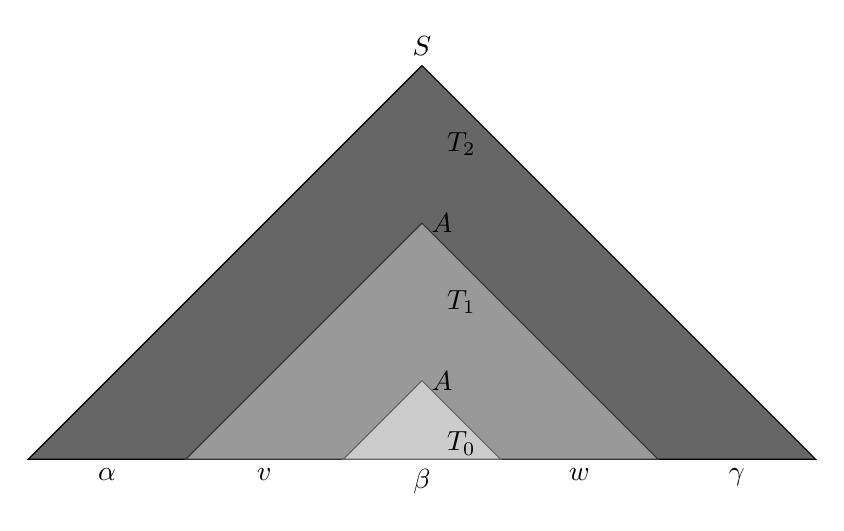
\begin{tikzpicture}
    \node (q0) at (0,0) [above]{$S$};
    \fill[color = black!60] (0,0) -- (-5,-5) -- (5,-5) -- (0,0);
    \draw (0,0) -- (-5,-5) -- (5,-5) -- (0,0);
    \node (q1) at (0.5,-1) {$T_2$};
    \node (q2) at (0,-2) [right]{$A$};
    \fill[color = black!40] (0,-2) -- (-3,-5) -- (3,-5) -- (0,-2);
    \draw[color = black!80] (0,-2) -- (-3,-5) -- (3,-5) -- (0,-2);
    \node (q3) at (0.5,-3) {$T_1$};
    \node (q4) at (0,-4) [right]{$A$};
    \fill[color = black!20] (0,-4) -- (-1,-5) -- (1,-5) -- (0,-4);
    \draw[color = black!60] (0,-4) -- (-1,-5) -- (1,-5) -- (0,-4);
    \node (q5) at (0.5,-4.8) {$T_0$};
    \node (q6) at (-4,-5) [below]{$\alpha$};
    \node (q7) at (-2,-5) [below]{$v$};
    \node (q8) at (0,-5) [below]{$\beta$};
    \node (q9) at (2,-5) [below]{$w$};
    \node (q10) at (4,-5) [below]{$\gamma$};
  \end{tikzpicture}

  \vspace{0.2cm}
  \hrule

  \vspace{0.2cm}
  \caption{Illustration du lemme d'itération}
\end{figure}

\subsection{Ambiguïté et propriété universelle}

Un problème se présente cependant, avec les arbres de dérivation. Dans le cas
des dérivations d'un mot, de la forme $\nTA\rtClot{\to} \varwd$, on sait qu'il
existe en général de nombreuses dérivations, mais qu'en est-il des arbres de
dérivation ?

Une grammaire peut en fait, ou non, posséder un unique arbre de dérivation pour
chaque mot~: c'est ce qu'on appelle une grammaire non ambiguë.

\begin{definition}[Ambiguïté]
  Soit $\ABA$ un alphabet et $\varGG$ une grammaire sur $\ABA$. On dit que
  $\varGG$ est ambiguë lorsqu'il existe deux arbres de dérivation sur $\varGG$
  distincts mais de même frontière. On dit qu'un langage algébrique $\varLL$ est
  inhéremment ambigu s'il n'existe aucune grammaire non ambiguë engendrant
  $\varLL$.
\end{definition}

La notion d'ambiguïté, ou plutôt de non ambiguïté, nous permet de définir une
propriété universelle, analogue au \cref{thm.PU.ind}.

\begin{proposition}[Propriété universelle d'une grammaire non ambiguë]
  \label{prop.PU.gram}
  Soit $\ABA$ un alphabet et $\varGG=(\ABB,\to,\StGr)$ une grammaire non ambiguë
  sur $\ABA$. Soit un ensemble $X$ et une famille
  $(f_{\nTA,\varwd})_{(\nTA,\varwd) \in \mathord{\to}}$ de
  fonctions telles que pour tout $(\nTA,\varwd) \in \mathord{\to}$, en
  décomposant $\varwd = \varwd_1\nTA_1\cdots\varwd_k\nTA_k\varwd_{k+1}$, on a
  $\makeFunName{f_{\nTA,\varwd}}{X^k}{X_{\nTA}}$.
  Il existe alors une unique fonction $f : \varLL_{\varGG} \to X$ telle que pour
  toute règle $\nTA \to \varwd_1\nTA_1\cdots \nTA_k\varwd_{k+1}$ et mots
  $\varwv_1,\ldots,\varwv_k\in\toStA$ tels que
  $\nTA_i \rtClot{\to} \varwv_i$, on a l'égalité
  \[f(\varwd_1\wdPt \varwv_1\wdPt\cdots\wdPt \varwv_k \varwd_{k+1}) =
  f_{\nTA,\varwd_1\nTA_1\cdots \nTA_k\varwd_{k+1}}(f(\varwv_1),\ldots,f(\varwv_k))\]
\end{proposition}

\begin{proof}
  On applique simplement le \cref{thm.ind.rec.gen} à la famille de fonctions
  $(f_{\nTA,\varwd})$, et on applique la fonction ainsi construite~: pour
  un mot $\varwd\in\varLL_{\varGG}$, il existe par non ambigüité un unique arbre
  de dérivation $T\in\derTr(\StGr)$ tel que $\front(T) = \varwd$, et on
  associe alors $f(\varwd) = f_{\StGr}(T)$.
\end{proof}

\begin{remark}
  On peut bien sûr construire des familles de fonctions non homogènes, dans
  lesquels chaque non terminal donne une fonction vers un ensemble différent,
  mais la propriété universelle serait encore plus lourde à écrire.
\end{remark}

Nous profitons de ces définitions pour donner la bijection de Cantor, qui
permet d'encoder des données finies grâce à des entiers. On va ici en faire
usage pour donner un premier cas d'utilisation de notre propriété universelle
avec une première version de codage de Gödel.

\begin{definition}[Bijection de Cantor \cite{Cantor1877}]\label{def.bij.Cantor}
  On appelle bijection de Cantor, ou polynôme de Cantor, la fonction
  \[\makeFunIso{\BijCB}{\bN\times\bN}{\bN}
               {(n,m)}{\displaystyle\left(\sum_{k = 1}^{n+m} k\right)+m}
  \]
\end{definition}

\begin{exercise}
  Montrer que la bijection de Cantor est effectivement une bijection, et qu'elle
  est croissante strictement en chacun de ses arguments.
\end{exercise}

L'intérêt de cette fonction est de nous donner un encodage des paires d'entiers
avec les entiers eux-mêmes. On peut en fait généraliser cette idée avec les
$k$-uplets d'entiers, et même les listes d'entiers.

\begin{definition}\label{def.bij.pairing}
  On définit la \ordinalnumeralfeminin{$n$} bijection, $\BijCn$, par
  récursion sur $n$~:
  \begin{itemize}
  \item la bijection $\BijCP{1} : \bN \cong \bN$ est définie par
    l'identité.
  \item si $\BijCn$ est définie, alors on définit
    \[\makeFunIso{\BijCP{n+1}}{\bN^{n+1}}{\bN}
                 {(p_1,\ldots,p_{n+1})}{\BijCB(\BijCn(p_1,\ldots,p_n),p_{n+1})}\]
  \end{itemize}

  On définit aussi la bijection $\makeFunNameIso{\BijCs}{\toSt{\bN}}{\bN}$
  par récursion sur les listes~:
  \begin{itemize}
    \begin{minipage}{0.3\textwidth}
    \item $\BijCs(\Ewd) = 0$
    \end{minipage}
    \begin{minipage}{0.65\textwidth}
    \item $\BijCs(\varwd\wdPt n) = 1 + \BijCB(\BijCs(\varwd),n)$
    \end{minipage}
  \end{itemize}
\end{definition}

\begin{exercise}
  Montrer que $\BijCn$ et $\BijCs$ sont des bijections croissantes strictement
  en chaque coordonnée.
\end{exercise}

\begin{notation}
  On notera en général $\langle n,m\rangle$ pour $\BijCB(n,m)$, et de même
  $\langle n_1,\ldots,n_p\rangle$ pour $\BijCP{n}(n_1,\ldots,n_p)$.
\end{notation}

\begin{definition}[Codage de Gödel - version 1 \cite{cori1993logique}]
  Soit $\ABA$ un alphabet et $\varGG=(\ABB,\to,\StGr)$ une grammaire non ambiguë
  sur $\ABA$. Pour chaque $\nTA \in \ABB$, on numérote les règles
  $(\nTA,\varwd) \in \mathord{\to}$ pour les ordonner, on note $e(\nTA,\varwd)$
  le numéro de la règle $\nTA\to \varwd$. Soit
  $\varwd = \varwd_1\nTA_1\cdots \nTA_n\varwd_{n+1}$, on définit
  \[f_{\nTA,\varwd}(x_1,\ldots,x_n)\defeq
  \langle e(\nTA,\varwd),x_1,\ldots,x_n\rangle\]
  La fonction obtenue est ce qu'on appelle un codage de Gödel de
  $\varLL_{\varGG}$~:
  \[\makeFunName{\godcod{\tok}}{\varLL_{\varGG}}{\bN}\]
\end{definition}

\begin{example}
  On fixe une signature du premier ordre $\Sign$ et un ensemble de variables
  du premier ordre $\Var$. On peut définir les formules sur la signature $\Sign$
  par la grammaire suivante~:
  \begin{align*}
    \StGr &\inddefeq \forall x, \StGr \mid \exists x, \StGr\mid \Imp\\
    \Imp &\inddefeq \Disj \to \Imp \mid \Disj\\
    \Disj &\inddefeq \Conj \lor \Disj \mid \Conj\\
    \Conj &\inddefeq \Atom \land \Disj \mid \Atom\\
    \Atom &\inddefeq \lnot \Atom \mid \top \mid \bot \mid \Term = \Term \mid
    R^p(\Term,\ldots,\Term)\mid (\StGr)\\
    \Term &\inddefeq x \mid f^p(\Term,\ldots,\Term)
  \end{align*}
  où $x \in \Var$, $R^p$ décrit l'ensemble des symboles de relation
  d'arité $p$ et $f^p$ les symboles de fonctions d'arité $p$. Les tuples
  $\Term,\ldots,\Term$ sont des $p$-uplets~: en particulier pour $p = 0$ on a
  simplement $R^0$ (respectivement $f^0$).
  
  On peut vérifier que la grammaire est sans ambiguïté. Ainsi, pour une formule
  $\varFF$ donnée, on peut lui associer un entier naturel $\godcod\varFF$, en
  prenant comme numérotation l'ordre dans lequel on a présenté les règles venant
  d'un même non terminal.

  En particulier, lorsque $\Sign$ est la signature de l'arithmétique
  $\SignP{\Arith}$ dont nous avons parlé dans le \cref{chp.logpred}, on peut de
  plus associer à une formule $\varFF$ son code de Gödel $\godcod\varFF$, puis
  le terme dans le langage de l'arithmétique $\Ss^{\godcod\varFF}0$. On a ainsi une
  façon de représenter une formule de l'arithmétique à l'intérieur même de
  l'arithmétique. Nous verrons que ce processus est au c\oe ur des théorèmes
  d'incomplétude de Gödel.
\end{example}

\begin{remark}
  Le terme \og codage de Gödel\fg sert à désigner une fonction des formules
  logiques dans les entiers (ou, plus généralement, d'un ensemble d'objets
  syntaxiques dans les entiers). Dans notre cas, nous avons défini une fonction
  plus générale, mais il reste que cette fonction, dans le cas particulier de
  l'arithmétique, correspond à nos attentes. Cependant, nous n'allons pas
  faire usage de ce codage, car nous aurons l'occasion d'en définir un plus
  pratique sur le long terme. En effet, dans le \cref{chp.recur}, nous allons
  définir un codage de Gödel en prouvant en plus qu'il est calculable (en un
  sens que nous préciserons) et que les opérations les plus basiques effectuées
  sur ce codage sont aussi calculables.

  Relevons qu'historiquement, le premier codage de Gödel dans son article
  \cite{Godel1931-GDEBFU} utilisait la décomposition en facteurs premiers, pour
  encoder un tuple $(n_1,\ldots,n_k)$ par l'entier
  $2^{n_1}\times 3^{n_2}\times\cdots \times p_k^{n_k}$ où $(p_n)_{n \in \bN}$
  est l'énumération canonique des nombres premiers.
\end{remark}

\begin{remark}
  Dans notre description des propositions, nous avons un ensemble infini de
  symboles avec $x \in \Var$. Pour correspondre à notre paradigme où les
  règles sont en nombre fini, il suffit de considérer $x$ comme un symbole non
  terminal et la règle
  \[x \inddefeq x_0\mid x_{\Ss}(x)\]
  décrivant une variable initiale $x_0$ et une fonction injective non surjective
  $x_{\Ss} : \Var \to \Var$. Ainsi la variable $x_n$ est remplacée par la
  variable $(x_{\Ss})^n(x_0)$ et on a alors bien un langage algébrique. Cela
  nous donne d'ailleurs un codage plus explicite des termes (les expressions
  dérivées de $\Term$ dans notre grammaire).
\end{remark}

\section{Automates à pile}

Dans cette section, nous présentons la notion d'automates à pile. Nous avons vu
dans le chapitre précédent que les automates finis (déterministes ou non
déterministes) reconnaissent exactement les langages réguliers. Les automates à
pile, eux, reconnaissent exactement les langages algébriques.

La première sous-section est dédiée aux définitions, et en particulier au cas de
l'acceptation, car plusieurs possibilités existent pour définir l'acceptation
d'un mot par un automate à pile. Nous verrons dans la seconde sous-section les
conséquences de ces automates, en particulier un théorème de clôture et le cas
des automates à pile déterministes.

Précisons dès maintenant que si nous étudions le cas des automates à pile
déterministes, cela est dû au fait que ceux-ci ne sont pas équivalents aux
automates à pile non déterministes (contrairement au cas des automates finis).
Les automates déterministes reconnaissent une sous-classe stricte de la classe
des langages algébriques (qui, eux, sont reconnus par les automates à pile non
déterministes). On considère donc par défaut les automates comme non
déterministes.

\subsection{Premières définitions}

Un automate à pile peut se voir comme un automate fini auquel on adjoint une
liste de symboles que l'automate peut lire pour avoir une forme de mémoire.
Cette liste de symboles fonctionne suivant le principe LIFO
(\foreignexpr{last in, first out}), ce qui correspond à la notion informatique
de pile (d'où le nom)~: le symbole lu est le dernier symbole ajouté.

\begin{definition}[Automate à pile]
  Soit un alphabet $\ABA$. Un automate à pile sur $\ABA$ est la donnée d'un
  $5$-uplet $(\varQQ,\varqZ,\ABB,\varla_0,\mathord{\varRR})$ où~:
  \begin{itemize}
    \begin{minipage}{0.45\textwidth}
    \item $\varQQ$ est l'ensemble (fini) d'états
    \item $\varqZ \in \varQQ$ est l'état initial
    \end{minipage}
    \begin{minipage}{0.45\textwidth}
    \item $\ABB$ est l'alphabet de pile
    \item $\varla_0 \in \ABB$ est le symbole initial
    \end{minipage}
  \item 
    $\mathord{\varRR} \subseteq \varQQ \times \ABB\times
    (\ABA\cup \{\Ewd\})\times \varQQ \times \toStB$
    est la relation de transition. On notera
    $\varq,\varla \xrightarrow{\varlb} \varq',\varwd$ pour signifier
    $(\varq,\varla,\varlb,\varq',\varwd) \in \mathord{\varRR}$ et on appellera
    $\varlb$ l'étiquette de la transition.
  \end{itemize}
\end{definition}

\begin{figure}[t]
  \centering
  \begin{tikzpicture}[node distance = 2cm, on grid, auto]
    \node[state, initial] (q_0) {$\varqZ$};
    \path[->,>=latex]
    (q_0) edge [loop right] node
         {$\genfrac{}{}{0pt}{0}{*,0,**}{*,1,\Ewd}$} ();
  \end{tikzpicture}

  \vspace{0.2cm}
  \hrule

  \vspace{0.2cm}
  \caption{Exemple d'automate à pile}
  \label{fig.auto.pile1}
\end{figure}

\begin{notation}
  Comme dans le cas des automates finis, on considère par défaut qu'un automate
  dont on ne spécifie pas les composantes a pour ensemble d'état $\varQQ$, pour
  état initial $\varqZ$, et de plus que $\ABB$ est son alphabet de pile et
  $\varla_0$ son symbole initial.
\end{notation}

Contrairement au cas d'un automate fini déterministe ou non, utiliser un
automate à pile demande plus d'information que la simple donnée de l'automate.
Cela est dû au fait qu'un automate à pile se comportera différemment en fonction
de la pile qu'il lit. On introduit donc la notion de configuration, qui est une
description totale du calcul lors de l'exécution d'un automate à pile.

\begin{definition}[Configuration]
  Soit $\ABA$ un alphabet et $\varAuA$ un automate à pile sur $\ABA$. On appelle
  configuration sur $\varAuA$ une paire $(\varq,\varwd)$ où $\varq \in \varQQ$
  et $\varwd \in \toStB$.
\end{definition}

Comme dans le chapitre précédent, on définir une notion de trace, qui correspond
à un historique de l'exécution de l'automate.

\begin{definition}[Trace de l'exécution d'un automate à pile]
  Soit $\ABA$ un alphabet et $\varAuA$ un automate à pile sur $\ABA$.
  On appelle trace sur $\varAuA$ une suite finie $(C_p)$ de
  configurations telle que, pour tout indice $p$ où $C_p$ et $C_{p+1}$ sont
  définies, en notant $C_p = (\varq,\varwd)$ et $C_{p+1} = (\varq',\varwv)$, on
  peut trouver deux lettres $\varla,\varlb$ et deux mots $\varwd',\varwv'$ tels
  que
  \[\begin{cases}
  \varwd = \varla \varwd'\\
  \varwv = \varwv'\varwd'\\
  \varq,\varla \xrightarrow{\varlb} \varq',\varwv'
  \end{cases}\]
  
  Soit une trace $(C_p)_{p = 0,\ldots,k}$. On dit que cette trace est valide pour
  un mot $u$ si $C_0 = (q_0,\alpha_0)$ et si $u$ est la concaténation des
  étiquettes des transitions de la trace $(C_p)$. Plus généralement, la
  concaténation de ces étiquettes est appelée l'étiquette de la trace de
  $(C_p)$, l'état de la configuration $C_0$ est l'état de départ et son mot est
  le mot de départ.
\end{definition}

\begin{example}\label{ex.pile.trace}
  L'exemple de la \cref{fig.auto.pile1} nous fournit un automate à pile sur
  $\ABA = \btwo$. On donne en exemple une trace d'exécution du mot $011$
  par cet automate, en prenant comme symbole initial $*$~:
  \[(\varqZ,*) \xrightarrow{0} (\varqZ,**) \xrightarrow{1} (\varqZ,*)
  \xrightarrow{1} (\varqZ,\Ewd)\]
\end{example}

Remarquons que pour l'instant, si on a effectivement défini ce qu'est un calcul
sur un automate à pile, par le biais des traces, il nous manque un critère
permettant d'arrêter un calcul. Plus précisément, étant donnée une trace
$(C_p)_{k = 0,\ldots,k}$, nous n'avons pas de condition sur la dernière
configuration $C_k$ pour déclarer que la trace représente effectivement un
calcul qui se termine.

Plusieurs tels critères existent. Nous en donnons deux~:
\begin{itemize}
\item par état final~: on définit un ensemble $\varAF$ d'états finaux, et la
  trace termine si l'état $q_k$ appartient à l'ensemble $\varAF$~;
\item par pile vide~: la trace termine lorsque $\varwd_k = \Ewd$.
\end{itemize}

\begin{remark}
  Dans l'\cref{ex.pile.trace}, on peut déduire que $011$ est reconnu par pile
  vide par l'automate donné en \cref{fig.auto.pile1}.
\end{remark}

Ces deux critères définissent la même classe de langages reconnus (celle des
langages algébriques, comme on s'y attend).
Pour vérifier cela, on commence par définir la notion de fond de pile testable.

\begin{definition}[Fond de pile testable]
  Soit $\ABA$ un alphabet et $\varAuA$ un automate à pile. On dit que cet
  automate est à fond de pile testable s'il existe une partition
  $\ABB = \ABB_0 \sqcup \ABB_1$ telle que pour toute configuration accessible
  depuis la configuration $(\varqZ,\varla_0)$, c'est-à-dire toute configuration
  appartenant à une trace dont la configuration précédente est la configuration
  de départ, en notant cette configuration $(\varq,\varwd)$, alors
  $\varwd$ peut se décomposer en $\varwd'\varla$ où $\varwd' \in \ABB_0$ et
  $\varla \in \ABB_1$. Dit autrement, un fond de pile est testable si pour
  toute exécution de l'automate, il est toujours possible à partir du mot en
  tête de pile de savoir si la pile est réduite à une lettre ou non.
\end{definition}

\begin{proposition}
  Soit $\ABA$ un alphabet, et $\varAuA$ un automate sur $\ABA$. Alors il existe
  un automate à fond de pile testable reconnaissant le même langage que
  $\varAuA$, que $\varAuA$ reconnaisse par état final ou par pile vide.
\end{proposition}

\begin{proof}
  L'idée de la démonstration est de doubler l'alphabet $\ABB$~: on crée une
  nouvelle copie
  \[\ABB' \defeq \compr{\varla_{\bis}}{\varla \in \ABB}\]
  disjointe avec $\ABB$ de sorte que le fond de pile est toujours occupé par une
  lettre de $\ABB'$. Il nous suffit ensuite d'ajouter des transitions de sorte à
  garder en mémoire si la lettre correspond ou non à une lettre de fond de pile.
\end{proof}

\begin{theorem}
  Soit $\ABA$ un alphabet, un langage $\varLL$ est reconnu par un automate à
  pile par état final si et seulement s'il est reconnu par un automate à pile
  par pile vide.
\end{theorem}

\begin{proof}
  Le théorème contient deux parties~: on veut construire un automate à pile par
  état final à partir d'un automate à pile par pile vide, et inversement.

  On suppose donc, pour commencer, que le langage $\varLL$ est reconnu par un
  automate à pile à fond de pile testable par état final $\varAuA$. On veut
  maintenant construire un automate à pile par pile vide. Pour cela, on ajoute
  deux états $\varqP{+}$ et $\varqP{-}$ représentant respectivement le cas où on
  atteint un état final, et le cas où la pile se vide avant d'atteindre un état
  final.

  Dans le premier cas, on ajoute une transition de la forme
  $\varq,\varla\xrightarrow{\varlb}\varq{+},\Ewd$ pour chaque transition de la
  forme $\varq,\varla\xrightarrow{\varlb} \varq',\varwv$ où $\varq' \in \varAF$,
  ainsi que toutes les transitions
  $\varqP{+},\varla \xrightarrow{\Ewd} \varqP{+},\Ewd$,
  permettant ainsi de transformer une trace pour le premier automate en une
  trace du nouvel automate identique jusqu'à l'état final, remplacé par
  $\varqP{+}$ où la pile se vide alors.
  Pour le cas de $\varqP{-}$, on ajoute toutes les transitions
  $\varq,\varla \xrightarrow{\varlb} \varqP{-},\varla$ pour $\varla$ une lettre
  de fond de pile ne menant pas à un état final. Ainsi les traces sur l'automate
  initial sont associées soit à une trace vidant sa pile dans l'état
  $\varqP{+}$, soit par une trace bloquante en $\varqP{-}$ où aucune transition
  ne peut être exécutée mais où la pile n'est pas vide.

  Réciproquement, si le langage est reconnu par un automate à pile à fond de
  pile testable par pile vide, alors on peut ajouter un unique état final
  $\varqP{f}$ et une transition
  $\varq,\varla\xrightarrow{\varlb} \varqP{f},\varla$ pour toute lettre
  $\varla$ de fond de pile.
\end{proof}

\begin{remark}
  Avec la preuve précédente, il est direct d'en déduire aussi que la combinaison
  des deux critères d'arrêt donne encore un critère d'arrêt pour les automates
  à piles, qui engendre la même classe de langage.
\end{remark}

\begin{definition}[Langage reconnaissable par pile]
  Un langage $\varLL \subseteq \toStA$ est reconnaissable par automates à pile
  lorsqu'il existe un critère parmi ceux cités précédemment et un automate à
  pile $\varAuA$ tel que pour tout $\varwd \in \toStA$, $\varwd \in \varLL$ si
  et seulement s'il existe une trace valide pour $\varwd$ dont la dernière
  configuration est une configuration d'arrêt pour le critère choisi.
\end{definition}

Nous concluons maintenant la sous-section en montrant l'équivalence entre les
grammaires hors contextes et les automates à pile.

\begin{theorem}\label{thm.reco.alg}
  Soit $\ABA$ un alphabet. On a égalité entre la classe des langages
  algébriques et celle des langages reconnaissable par un automate à pile.
\end{theorem}

\begin{proof}
  Commençons par montrer qu'un langage algébrique est reconnaissable par un
  automate à pile pour le critère de pile vide et état final.

  Soit une grammaire $\varGG=\{\ABB,\{\nTA_i\to\varww_i\}_{i \in I},\StGr\}$, on
  construit l'automate $\varAuP{\varGG}$ suivant~:
  \begin{itemize}
    \begin{minipage}{0.65\textwidth}
    \item $\varQQ \defeq \{\varqZ\} \cup \{\varqP{f}\} \cup
      \compr{\varqP{i,j}}{i \in I, \varww \in \intervIntB{\wdl{\varww_i}}}$
    \end{minipage}
    \begin{minipage}{0.3\textwidth}
    \item $\ABB_{\varAuP{\varGG}} \defeq \ABA \cup \ABB$
    \end{minipage}
  \item le symbole initial est vide (quitte à créer une transition le
    supprimant au début de l'automate)
  \item l'unique état final est $\varqP{f}$
  \item la relation $\varRR$ est définie par les faits suivants~:
    \begin{itemize}
    \item on a une transition
      $\varqZ,\StGr\xrightarrow{\Ewd} \varqP{f},\Ewd$
    \item pour toute règle $\nTA_i \to \varww_i$, on ajoute les transitions
      (en considérant que $\varqP{i,0} = q_0$)
      \[\forall j < \wdl{\varww_i}, \varqP{i,j}, (\varww{i})_{\wdl{\varww_i}- j}
      \xrightarrow{\Ewd} \varqP{i,j+1},\Ewd\]
      ainsi que $\varqP{i,\wdl{\varww_i}},\Ewd\xrightarrow{\Ewd} \varqZ,\nTA_i$
    \item pour toute lettre $\varla \in \ABA$, on ajoute la transition
      \[\varqZ,\Ewd \xrightarrow{\varla} \varqZ,\varla\]
      (que l'on peut encoder par, pour tout symbole de pile $\varlb$,
      $\varqZ,\varlb\xrightarrow{\varla} \varqZ,\varla\varlb$)
    \end{itemize}
  \end{itemize}
  On ne montrera pas rigoureusement l'équivalence des deux langages, mais on
  donne une esquisse de preuve. D'abord,
  on remarque qu'une trace d'exécution valide est constituée d'alternances de
  deux types de blocs de configurations~:
  \begin{itemize}
  \item des blocs augmentant la taille de la pile, où toutes les transitions
    sont de la forme $\varqZ,\Ewd \xrightarrow{\varla}\varqZ,\varla$
  \item des blocs diminuant la taille de la pile, où le bloc commence à l'état
    $\varqZ$ puis dépile toutes les lettres correspondant au mot $\varww_i$
    d'une règle $\nTA_i \to \varww_i$, puis revient à l'état $\varqZ$ en
    empilant la lettre $\nTA_i$
  \end{itemize}
  Suite à cette alternance, on obtient une pile constituée uniquement par
  $\StGr$ sur l'état $\varqZ$, permettant d'aller à l'état $\varqP{f}$. Pour une
  dérivation d'un mot $\varwd$ depuis $\StGr$, on remarque qu'il est possible
  d'effectuer le parcourt de l'automate à l'envers~: si la première règle
  utilisée est $\StGr \to \varww$, alors on a un bloc de transitions de $\varqZ$
  à $\varqZ$ tel que la pile vaut d'abord $\varww$, puis finit par valoir
  $\StGr$. Ainsi, les dérivations correspondent à des traces valides, et
  inversement puisqu'un bloc va toujours correspondre à une dérivation.

  Montrons le sens réciproque. Pour cela, on utilise la méthode des triplets de
  Ginsburg \cite{ginsburg1966mathematical}. Soit un automate à pile $\varAuA$
  reconnaissant le langage $\varLL$ par pile vide. On suppose sans perte de
  généralité (quitte à ajouter des états et des transitions) que toute
  transition n'empile qu'au plus deux symboles.

  Pour tous états $\varq,\varq'$ et symbole de pile $\varla$, on définit
  $\varLL_{\varq,\varq',\varla}$ l'ensemble des mots $\varwd$ des tels qu'il existe
  un calcul valide pour $\varwd$ entre la configuration $(\varq,\varla)$ et la
  configuration $(\varq',\Ewd)$. On remarque que si
  $\varwd \in \varLL_{\varq,\varq',\varla}$, alors pour tout mot $\varww$, il existe
  un calcul valide pour $\varwd$ entre $(\varq,\varla \varww)$ et
  $(\varq',\varww)$. On donne les égalités~:
  \begin{align*}
    \varLL &=
    \displaystyle\bigcup_{\varq' \in \varQQ} \varLL_{\varqZ,\varq',\varla_0} \\
    \varLL_{\varq,\varq',\varla} &=
    \compr{\varlb}{\varq,\varla \xrightarrow{\varlb} \varq',\Ewd}
    \cup\displaystyle\bigcup_{\varq,\varla\xrightarrow{\varlb} \varq'',\varlc}
    \varlb\varLL_{\varq'',\varq',\varlc}
    \cup\bigcup_{\varq,\varla\xrightarrow{\varlb} \varqP{1},\varlc\varld}
    \varlb\varLL_{\varqP{1},\varqP{2},\varlc}\varLL_{\varqP{2},\varq',\varld}
  \end{align*}
  La première égalité signifie simplement que reconnaître par pile vide un mot
  $\varwd$ peut se réécrire en l'existence d'un calcul valide pour $\varwd$
  entre $(\varqZ,\varla_0)$ et $(\varq',\Ewd)$ pour un état $\varq'$.

  La seconde égalité, elle, contient trois termes. En effet, si l'on veut faire
  un calcul entre $(\varq,\varla)$ et $(\varq',\Ewd)$, trois cas sont
  possibles~:
  \begin{itemize}
  \item soit on supprime simplement la $\varla$ dans une transition d'étiquette
    $\varlb$~;
  \item soit on a une transition d'étiquette $\varlb$ jusqu'à une configuration
    $(\varq'',\varlc)$, puis un calcul de $(\varq'',\varlc)$ à $(\varq',\Ewd)$~;
  \item soit on a une transition d'étiquette $\varlb$ jusqu'à une configuration
    $(\varqP{1},\varlc\varld)$, puis un calcul de $(\varqP{1},\varlc,\varld)$ à
    $(\varqP{2},\varld)$, puis un calcul de $(\varqP{2},\varld)$ à
    $(\varq',\Ewd)$.
  \end{itemize}
  On peut ainsi construire naturellement une grammaire correspondant à ces
  langages~:
  \begin{itemize}
  \item $\ABB$ est pris comme l'ensemble des triplets $(\varq,\varq',\varla)$
  \item le non terminal de départ est $\StGr$ muni d'une transition vers chaque
    $\varLL_{\varqZ,\varq',\varla_0}$ pour $\varq' \in \varQQ$
  \item les transitions sont celles indiquées par la seconde équations (on
    remplace simplement les unions par des $+$ et le $=$ par une flèche $\to$)
  \end{itemize}
  Ainsi, une dérivation correspond naturellement à un calcul, et un calcul
  acceptant un mot correspond à une dérivation du mot dans cette grammaire.
\end{proof}

\subsection{Automates à pile déterministes}

Dans le \cref{chp.auto}, nous avons vu que les automates finis déterministes et
non déterministes sont équivalents quant au langage qu'ils reconnaissent. Dans
le cas des automates à pile, on va voir que cela n'est plus le cas.

Pour les automates finis, comme chaque étape de calcul correspond à la lecture
d'une lettre, le déterminisme ou non d'un automate se caractérise simplement par
le fait que sa relation de transition est fonctionnelle. Dans le cas présent,
cependant, cette distinction n'est pas aussi simple~: il est par exemple permis
d'utiliser des $\Ewd$-transitions dans un automate à pile déterministe, tant que
cette transition n'intervient pas sur un état où d'autres transitions avec des
lettres sont possibles (ceci pour permettre de mieux gérer l'empilement et le
dépilement).

\begin{definition}[Automate à pile déterministe]
  Un automate à pile $\varAuA = (\varQQ,\varqZ,\ABB,\varla_0,\varRR)$ sur un
  alphabet $\ABA$ est dit déterministe si pour chaque configuration
  $(\varq,\varla)$, l'une des deux conditions suivantes est vérifiée~:
  \begin{itemize}
  \item soit il existe une unique transition
    $\varq,\varla\xrightarrow{\Ewd} \varq',\varlb$ et il n'y a aucune transition
    $\varq,\varla\xrightarrow{\varlb} \varq',\varlc$ pour un
    élément $\varlb \in \ABA$
  \item soit il n'existe aucune transition de la forme
    $\varq,\varla\xrightarrow{\Ewd} \varq',\varlb$ et pour chaque
    $\varla \in \ABA$, il existe au plus une transition de la forme
    $\varq,\varla\xrightarrow{\varlb} \varq',\varlc$.
  \end{itemize}

  Un langage algébrique est dit déterministe s'il est reconnaissable par un
  automate à pile déterministe.
\end{definition}

La proposition principale qui justifie l'introduction de la version déterministe
des automates à pile est la suivante~:

\begin{proposition}[Non ambiguïté des langages algébriques déterministes]
  Un langage $\varLL\subseteq \toStA$ algébrique déterministe est un langage non
  ambigu.
\end{proposition}

\begin{proof}
  En utilisant la méthode des triplets de Ginsburg sur l'automate à pile
  reconnaissant le langage, on obtient une correspondance entre les calculs de
  l'automate et les dérivations de la grammaire. Il nous suffit donc d'avoir
  l'unicité des calculs de l'automate~: l'obstacle majeur à cette unicité est la
  possibilité de faire des $\Ewd$-transitions à la fin du calcul, ou une
  infinité d'$\Ewd$-transitions au milieu du calcul. Il est possible de modifier
  l'automate pour assurer ce fait, mais nous l'admettons ici (la preuve peut se
  trouver dans \cite{carton2008langages} à la proposition 2.77).
\end{proof}

\newpage

\section{Exercices et problèmes}

\subsection{Exercices}

\begin{exercise}[Un lemme classique sur les langages algébriques]
  Montrer que si $\varLL$ est un langage algébrique et $\varLL'$ est un
  langage rationnel, alors $\varLL \cap \varLL'$ est un langage
  algébrique.

  En supposant $\varLL'$ algébrique, le résultat est-il toujours vrai ?
\end{exercise}

\begin{exercise}[Complémentaire d'un langage déterministe]
  Montrer que la classe des langages algébriques déterministes est stable par
  complémentaire.
\end{exercise}
